\documentclass[11pt]{article}

\usepackage{amsmath}
\usepackage{amssymb}
\usepackage[margin=0.72in]{geometry}
\usepackage{booktabs}
\usepackage{circuitikz}
\usepackage{enumitem}
\usepackage{fancyhdr}
\usepackage{graphicx}
\usepackage[table]{xcolor}
\usepackage{hyperref}
\usepackage{listings}
\usepackage{microtype}
\usepackage{tabularx}
\usepackage{tikz}
\usepackage{titlesec}
\graphicspath{{docs/lessons/assets/}{../assets/}}

\definecolor{AdkBlue}{HTML}{24577A}
\definecolor{AdkRed}{HTML}{A23B32}
\definecolor{AdkGreen}{HTML}{39734C}
\definecolor{AdkGray}{HTML}{F0F2F3}
\definecolor{CodeGray}{HTML}{F7F7F7}

\hypersetup{colorlinks=true,linkcolor=AdkBlue,urlcolor=AdkBlue}
\pagestyle{fancy}
\fancyhf{}
\lhead{\textsc{ADK Lesson 002}}
\rhead{Two independent LEDs}
\cfoot{\thepage}
\setlength{\headheight}{14pt}
\setlength{\parindent}{0pt}
\setlength{\parskip}{5pt}
\setlist{nosep,leftmargin=1.45em}
\titleformat{\section}{\Large\bfseries\color{AdkBlue}}{\thesection}{0.5em}{}
\titleformat{\subsection}{\large\bfseries\color{AdkBlue}}{\thesubsection}{0.5em}{}

\lstdefinestyle{adkcpp}{
  language=C++,
  backgroundcolor=\color{CodeGray},
  basicstyle=\ttfamily\small,
  keywordstyle=\color{AdkBlue}\bfseries,
  commentstyle=\color{AdkGreen},
  stringstyle=\color{AdkRed},
  columns=fullflexible,
  keepspaces=true,
  showstringspaces=false,
  frame=single,
  rulecolor=\color{black!20},
  breaklines=true,
  tabsize=4
}

\newcommand{\checkbox}{\(\square\)}
\newcommand{\blank}[1]{\rule{#1}{0.4pt}}
\newcommand{\SI}[2]{\ensuremath{#1\,\mathrm{#2}}}
\newcommand{\si}[1]{\ensuremath{\mathrm{#1}}}
\newcommand{\volt}{V}
\newcommand{\ohm}{\Omega}
\newcommand{\milli}{m}
\newcommand{\ampere}{A}
\newcommand{\second}{s}
\newcommand{\warningbox}[1]{%
  \begin{center}
  \fcolorbox{AdkRed}{AdkRed!6}{\parbox{0.91\linewidth}{\textbf{\color{AdkRed}Safety checkpoint.} #1}}
  \end{center}}
\newcommand{\evidencebox}[1]{%
  \begin{center}
  \fcolorbox{AdkBlue}{AdkBlue!5}{\parbox{0.91\linewidth}{#1}}
  \end{center}}

\begin{document}

\begin{center}
  {\Huge\bfseries Two Independent LEDs}\\[4pt]
  {\Large Pins 4 and 7 on the Arduino Mega 2560}\\[8pt]
  \textit{Build deliberately, predict first, and support every claim with repeated evidence.}
\end{center}

\begin{tabularx}{\linewidth}{@{}>{\bfseries}l X >{\bfseries}l X@{}}
Lesson & 002 & Time & 70--100 minutes\\
Level & First external-output circuit & Board & Arduino Mega 2560\\
Outcome & Independently command and verify two current-limited LEDs & Evidence & Prediction, measurements, three trials, CER\\
\end{tabularx}

\section{Why this circuit matters}

The built-in LED hides its wiring. Here, you make every electrical choice: output pin,
current-limiting resistor, LED polarity, and return path. Two branches then reveal an
important idea: components can share ground and still be controlled independently.
That pattern expands naturally to status panels, traffic signals, displays, and
diagnostic indicators.

\subsection*{Learning targets}

By the end, you can:

\begin{itemize}
  \item trace each complete path from a Mega output pin to ground;
  \item identify an LED's anode and cathode before energizing;
  \item calculate a safe resistor value and estimate branch current;
  \item distinguish a wiring observation from a software claim;
  \item collect repeated evidence that pins 4 and 7 control separate branches;
  \item explain how an RAII component can leave an output in a safe state.
\end{itemize}

\section{Roles and safety}

Work alone or use two roles. Swap roles after the first successful trial.

\begin{description}[style=nextline]
  \item[Builder / operator] Keeps all power sources disconnected while changing wiring,
  reads resistor bands, places parts, and announces before power is applied.
  \item[Verifier / recorder] Traces the exact schematic, checks LED polarity and
  shared ground, records predictions and measurements, and calls ``stop'' if a
  connection differs from the schematic.
\end{description}

\warningbox{Disconnect \emph{all} power sources---USB, barrel-jack supply,
battery, programmer, and powered external modules---before inserting, moving,
or removing any wire or component. Never connect an LED directly between an output and ground:
each LED needs its own series resistor. Do not connect pins 4 and 7 together.
If a component becomes warm, an LED is unexpectedly bright, or the board resets,
disconnect power immediately.}

\textbf{Required:} Mega 2560, USB cable, breadboard, two LEDs (preferably visibly
different colors), two \SI{330}{\ohm} resistors, jumper wires, and a multimeter.
Use the \SI{20}{\volt} DC range (or auto-range) for voltage. Current measurement is
optional and must be done only with an instructor-approved series connection;
never place a meter in current mode directly across a pin and ground.

\section{Predict before building}

The sketch alternates the LEDs: red on/blue off, then red off/blue on. Complete
these predictions before touching the hardware.

\begin{tabularx}{\linewidth}{@{}c c c X@{}}
\toprule
Pin 4 level & Pin 7 level & Predicted visible result & Why?\\
\midrule
HIGH & LOW  & \rule{2.2in}{0.4pt} & \rule{2.3in}{0.4pt}\\[10pt]
LOW  & HIGH & \rule{2.2in}{0.4pt} & \rule{2.3in}{0.4pt}\\[10pt]
LOW  & LOW  & \rule{2.2in}{0.4pt} & \rule{2.3in}{0.4pt}\\
\bottomrule
\end{tabularx}

\textbf{De-energized-state prediction:} With all power disconnected, what should each LED
do? \blank{1.0in} Why can an LED not remain lit from these pin branches?
\blank{2.6in}

\textbf{Fault prediction:} If the blue LED is reversed but every other connection
is correct, predict what red and blue will do: \blank{4.0in}

\section{Two drawings, two jobs}

\begin{figure}[ht]
  \centering
  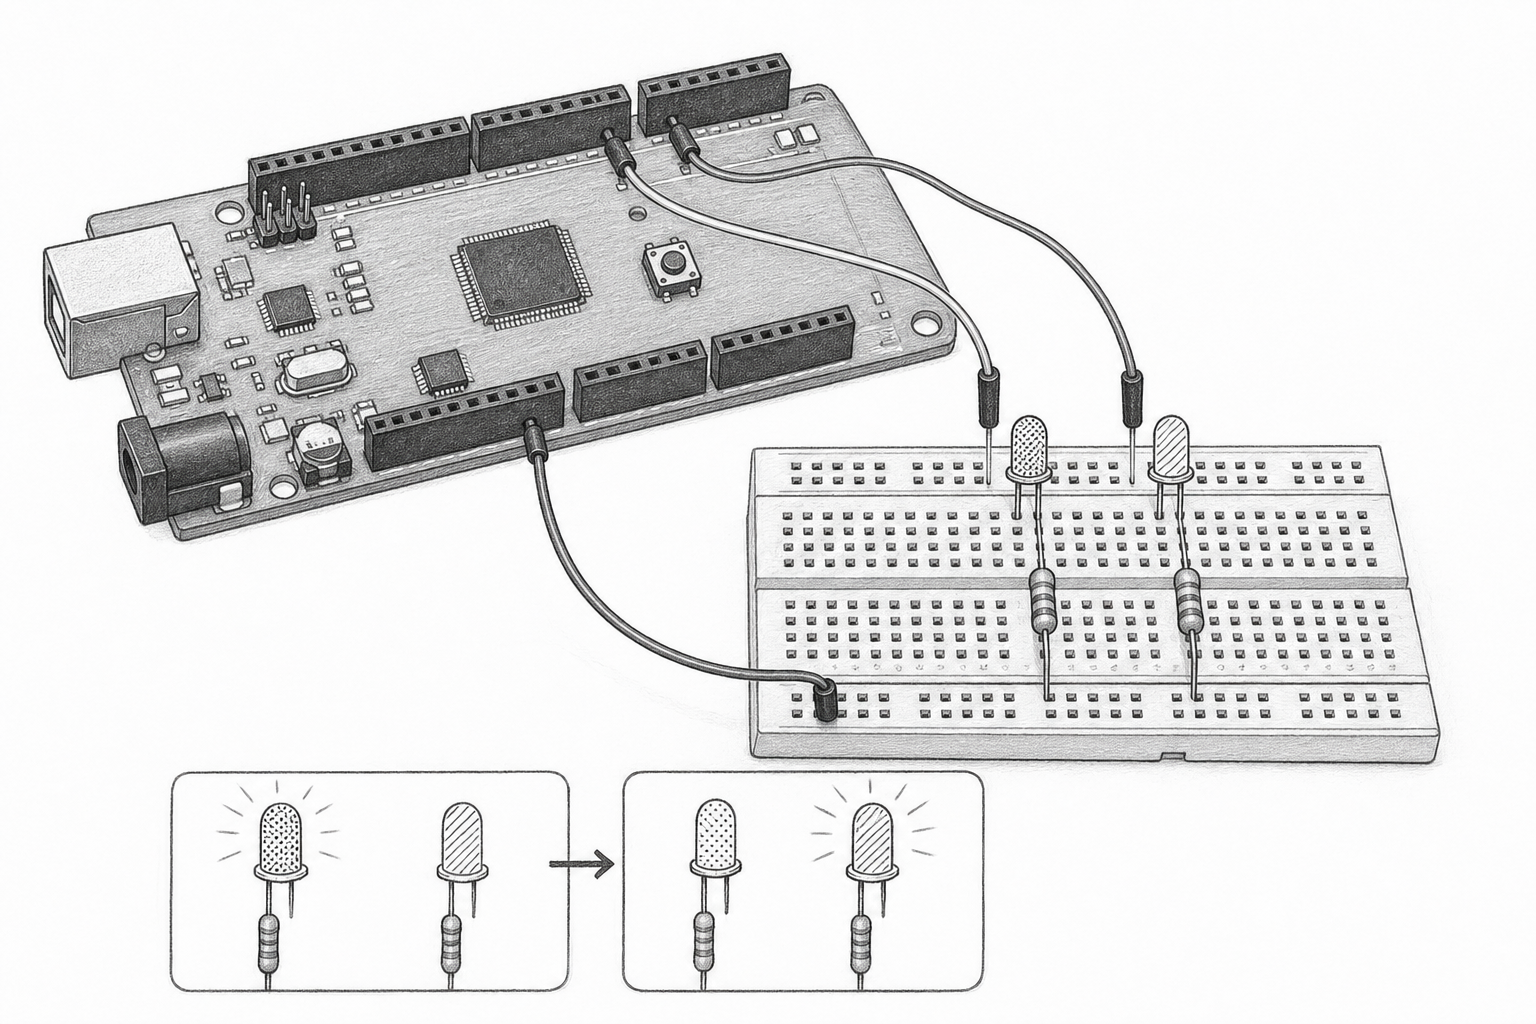
\includegraphics[width=0.82\linewidth]{002-two-leds-pencil.png}
  \caption{Conceptual orientation only. This pencil drawing communicates the idea
  of two LEDs, but it is \textbf{not literal wiring guidance}. It may simplify
  breadboard rows, pin positions, polarity, or resistor placement. Build from the
  exact schematic and connection table below.}
\end{figure}

\clearpage
\subsection{Exact electrical schematic}

\begin{center}
\begin{circuitikz}[american voltages]
  \draw
    (0,3) node[left]{Mega D4} to[short,o-] (1,3)
    to[R,l={$R_1=330\,\Omega$}] (3.3,3)
    to[leD,l={$LED_1$ red}] (5.7,3)
    -- (6.5,3) -- (6.5,0) node[ground]{};
  \draw
    (0,1.25) node[left]{Mega D7} to[short,o-] (1,1.25)
    to[R,l={$R_2=330\,\Omega$}] (3.3,1.25)
    to[leD,l={$LED_2$ blue}] (5.7,1.25)
    -- (6.5,1.25);
  \node[align=left,anchor=west] at (7.2,2.2)
    {\textbf{Two separate branches}\\
     Each branch has its own resistor.\\
     Both cathodes return to Mega GND.};
\end{circuitikz}
\end{center}

Conventional current flows from a HIGH output, through that branch's resistor,
through the LED from anode to cathode, and back through GND. On a common through-hole
LED, the longer lead is usually the anode; the flat edge and shorter lead usually
mark the cathode. Verify the part itself because leads may have been trimmed.

\begin{center}
\begin{tabular}{@{}llll@{}}
\toprule
From & Through & To & Verification\\
\midrule
Mega D4 & \(R_1=\SI{330}{\ohm}\), then red LED anode & red cathode to GND & branch 1 only\\
Mega D7 & \(R_2=\SI{330}{\ohm}\), then blue LED anode & blue cathode to GND & branch 2 only\\
\bottomrule
\end{tabular}
\end{center}

\textbf{Important breadboard rule:} The resistor and LED must be in series, not
merely near each other. Use a continuity check with power disconnected if the
breadboard's connected rows are unfamiliar.

\section{Choose the resistor with a calculation}

The resistor absorbs the voltage not dropped by the LED. Estimate branch current:

\[
 I=\frac{V_{\text{pin}}-V_f}{R}.
\]

Using an approximate \SI{5}{\volt} HIGH and \SI{330}{\ohm}:

\[
 I_{\text{red}}\approx\frac{\SI{5}{\volt}-\SI{2.0}{\volt}}
 {\SI{330}{\ohm}}=\SI{9.1}{\milli\ampere},
 \qquad
 I_{\text{blue}}\approx\frac{\SI{5}{\volt}-\SI{3.0}{\volt}}
 {\SI{330}{\ohm}}=\SI{6.1}{\milli\ampere}.
\]

These are pre-power estimates: actual pin HIGH voltage and LED forward voltage vary. A
\SI{330}{\ohm} resistor is deliberately conservative and normally provides a
clearly visible result without chasing maximum brightness.

\textbf{Pre-power calculation for your parts:} Use a datasheet value or reasonable
color-based estimate for \(V_f\). Do not try to measure \(V_f\) until the inspected,
current-limited circuit is safely energized.

\begin{tabularx}{\linewidth}{@{}l c c c X@{}}
\toprule
Branch & Assumed \(V_{\text{pin}}\) & Assumed LED \(V_f\) & \(R\) & Predicted \(I\)\\
\midrule
D4 / LED 1 & \blank{0.7in} & \blank{0.7in} & \blank{0.7in} & \blank{1.1in}\\[8pt]
D7 / LED 2 & \blank{0.7in} & \blank{0.7in} & \blank{0.7in} & \blank{1.1in}\\
\bottomrule
\end{tabularx}

\section{De-energized build procedure}

\begin{enumerate}
  \item \textbf{Disconnect all power.} Confirm: \checkbox\ USB disconnected;
  \checkbox\ no barrel/battery/programmer/module power; \checkbox\ board power LED off.
  \item Identify D4, D7, and a GND pin on the printed Mega labels. Do not infer
  positions from the pencil drawing.
  \item Read both resistor color codes and verify approximately
  \SI{330}{\ohm} with the meter if available.
  \item Build the D4 branch exactly as the schematic shows.
  \item Build the D7 branch exactly as the schematic shows.
  \item Trace aloud: ``D4, resistor, LED anode-to-cathode, ground,'' then repeat
  for D7.
  \item Check there is no wire joining D4 to D7 and no branch bypassing a resistor.
  \item Ask the verifier to initial the independent inspection: \blank{0.8in}.
\end{enumerate}

\evidencebox{\textbf{Power-on gate:} Do not connect any power source until every
item above is checked. A circuit that is unpowered is the correct state for inspection,
continuity tests, and changes.}

\section{Software: alternate the two outputs}

The current repository example for this lesson expresses each LED as a component:

\begin{lstlisting}[style=adkcpp]
#include <adk.h>

adk::led::Mono red  (4);
adk::led::Mono blue (7);

void setup()
{
    adk::initialize();
}

void loop()
{
    // A one-second dwell gives a DMM time to settle.
    constexpr auto intervalMs = 1000;

    red .on  ();
    blue.off ();
    delay(intervalMs);

    red .off ();
    blue.on  ();
    delay(intervalMs);
}
\end{lstlisting}

For this measurement exercise, set the supplied example's interval to
\SI{1000}{\milli\second} before uploading. Related member calls align their
parentheses so state transitions can be compared quickly.

\subsection{RAII and the component boundary}

The sketch should say \emph{what} the red and blue components do, while the library
owns \emph{how} a pin is configured and returned to a safe state. The intended
component contract uses a \texttt{struct}, normalized CamelCase names, out-of-line
implementation, explicit fallible initialization, and automatic cleanup:

\begin{lstlisting}[style=adkcpp]
struct Mono
{
    explicit Mono (PinId pin) noexcept;
             ~Mono() noexcept;

    Result initialize  () noexcept;
    void   shutdown    () noexcept;
    bool   initialized () const noexcept;

    void   on          () noexcept;
    void   off         () noexcept;
};
\end{lstlisting}

\warningbox{\textbf{Planned API, not current executable API:} the lifecycle
interface above is a design target and is not yet implemented by this lesson's
library. Do not copy it into the sketch expecting it to compile. The executable
example currently uses \texttt{adk::initialize()} and the available
\texttt{Mono::on()/off()} calls.}

\texttt{begin()} and \texttt{end()} are avoided because those names conventionally
describe iterator boundaries. Internally, ADK does not throw. Nevertheless, RAII
means that if application code is compiled with exceptions and stack unwinding
occurs, \texttt{\(\sim\)Mono()} still calls an idempotent \texttt{shutdown()}.
For an LED, shutdown first commands the inactive level; a generic output can then
use a high-impedance policy. Constructors should establish an inert valid object;
\texttt{initialize()} should claim/configure hardware transactionally and report
failure as a \texttt{Result}. Implementation stays in a \texttt{.cpp} wherever
templates or compile-time evaluation do not require header definitions.

\textbf{Design prompt:} Why is a \texttt{Mono} best modeled as owning its output-pin
resource rather than borrowing an untracked global pin? \blank{4.2in}

\section{Observe, measure, repeat}

Connect USB only after the power-on gate. Build and upload the lesson with the
project's Arduino CLI wrapper, or open the supplied \texttt{lessons/002/002.ino}
using a Mega 2560 board selection. Confirm that its measurement dwell is
\SI{1000}{\milli\second}, then observe at least three complete red/blue cycles.

\subsection{Voltage measurements}

Keep the black probe on Mega GND. Touch the red probe to D4, then D7. Record a
representative HIGH and LOW. Do not let a probe bridge adjacent header pins.
Only after those measurements, measure LED forward voltage by placing probes
across a lit LED: red probe at the anode and black probe at the cathode.

\begin{tabularx}{\linewidth}{@{}l c c c X@{}}
\toprule
Quantity & Trial 1 & Trial 2 & Trial 3 & Pattern / notes\\
\midrule
D4 when red is on (\si{\volt})  & \blank{0.55in} & \blank{0.55in} & \blank{0.55in} & \blank{1.5in}\\[8pt]
D4 when red is off (\si{\volt}) & \blank{0.55in} & \blank{0.55in} & \blank{0.55in} & \blank{1.5in}\\[8pt]
D7 when blue is on (\si{\volt}) & \blank{0.55in} & \blank{0.55in} & \blank{0.55in} & \blank{1.5in}\\[8pt]
D7 when blue is off (\si{\volt})& \blank{0.55in} & \blank{0.55in} & \blank{0.55in} & \blank{1.5in}\\[8pt]
Red LED \(V_f\), while lit (\si{\volt}) & \blank{0.55in} & \blank{0.55in} & \blank{0.55in} & \blank{1.5in}\\[8pt]
Blue LED \(V_f\), while lit (\si{\volt}) & \blank{0.55in} & \blank{0.55in} & \blank{0.55in} & \blank{1.5in}\\
\bottomrule
\end{tabularx}

\subsection{Repeated behavioral evidence}

\begin{tabularx}{\linewidth}{@{}c c c c c X@{}}
\toprule
Cycle & D4 command & Red observed & D7 command & Blue observed & Cross-control or anomaly?\\
\midrule
1 & ON/OFF & \blank{0.5in} & OFF/ON & \blank{0.5in} & \blank{1.7in}\\[8pt]
2 & ON/OFF & \blank{0.5in} & OFF/ON & \blank{0.5in} & \blank{1.7in}\\[8pt]
3 & ON/OFF & \blank{0.5in} & OFF/ON & \blank{0.5in} & \blank{1.7in}\\
\bottomrule
\end{tabularx}

\textbf{Aggregate-current boundary:} The two branches would draw approximately
\(\SI{9.1}{\milli\ampere}+\SI{6.1}{\milli\ampere}
=\SI{15.2}{\milli\ampere}\) if both were on. The base alternation draws only one
branch at a time. Do not infer that any number of such branches may be added:
pin, port-group, and whole-MCU supply/ground limits all apply simultaneously.
Recalculate the worst-case sum, check the ATmega2560 and board limits, and use an
external driver and suitable power supply before scaling to many loads.

\textbf{De-energized-state observation:} Disconnect all power after the trials. Record
the visible state of both LEDs and compare it with the earlier prediction.

\medskip
\noindent\blank{0.98\linewidth}

\section{Troubleshooting by symptom}

Disconnect all power \emph{before} applying any wiring remedy.

\begin{tabularx}{\linewidth}{@{}
  >{\bfseries\raggedright\arraybackslash}p{0.22\linewidth}
  >{\raggedright\arraybackslash}X
  >{\raggedright\arraybackslash}X@{}}
\toprule
Symptom & Likely cause & De-energized check or controlled test\\
\midrule
One LED never lights &
LED reversed, open row, wrong pin, or damaged LED &
Check cathode/anode, trace that branch, continuity-test rows, then swap only the
LED with a known-good one.\\
\addlinespace
Both LEDs always match &
Pins or branches accidentally joined, or code addresses one pin twice &
Verify D4 and D7 are not connected; compare constructor pin numbers.\\
\addlinespace
LED is extremely bright or board resets &
Missing/bypassed resistor or short circuit &
Disconnect immediately; verify one \SI{330}{\ohm} resistor is in series in each branch.\\
\addlinespace
Sequence is reversed &
LED colors/branches were exchanged or prediction mapped pins incorrectly &
Trace from D4 and D7 rather than assuming physical left/right position.\\
\addlinespace
Flicker or intermittent light &
Loose lead, split breadboard rail, or poor ground &
Gently reseat with power off; continuity-test the common ground path.\\
\addlinespace
Upload succeeds but neither lights &
Missing ground, both LEDs reversed, wrong board/port, or initialization failure &
Confirm shared GND and polarity; verify Mega 2560 selection; inspect returned
initialization status when the interface exposes it.\\
\bottomrule
\end{tabularx}

\textbf{One-change rule:} Write the symptom, change exactly one variable, then
repeat the same observation. Otherwise a successful result does not identify the
cause.

\begin{tabularx}{\linewidth}{@{}X X X@{}}
\toprule
Observed symptom & One controlled change & Result / inference\\
\midrule
\rule{0pt}{18pt}\blank{2.0in} & \blank{2.0in} & \blank{2.0in}\\[12pt]
\blank{2.0in} & \blank{2.0in} & \blank{2.0in}\\
\bottomrule
\end{tabularx}

\section{Controlled extension: encode three states}

Only after the base circuit has three successful cycles, modify \emph{software
only} to display this repeating sequence:

\begin{enumerate}
  \item red on, blue off for \SI{500}{\milli\second};
  \item both on for \SI{500}{\milli\second};
  \item red off, blue on for \SI{500}{\milli\second};
  \item both off for \SI{500}{\milli\second}.
\end{enumerate}

Predict first, then implement. This isolates the changed variable: timing/state
logic changes while hardware remains fixed.

\begin{tabularx}{\linewidth}{@{}c c c c X@{}}
\toprule
State & Red command & Blue command & Observed correctly? & Evidence\\
\midrule
1 & on  & off & \checkbox & \blank{2.0in}\\[7pt]
2 & on  & on  & \checkbox & \blank{2.0in}\\[7pt]
3 & off & on  & \checkbox & \blank{2.0in}\\[7pt]
4 & off & off & \checkbox & \blank{2.0in}\\
\bottomrule
\end{tabularx}

\textbf{Optional engineering extension:} Replace one resistor with
\SI{680}{\ohm} while power is disconnected. Predict and compare brightness and
calculated current. Restore the original part afterward. Never replace it with a
jumper.

\section{Assessment}

\begin{enumerate}
  \item Draw arrows on the schematic showing conventional current when D4 is HIGH.
  Why is there no intended current in the D7 branch when D7 is LOW?
  \vspace{0.42in}
  \item A green LED has \(V_f=\SI{2.2}{\volt}\). Estimate current with a
  \SI{330}{\ohm} resistor and a \SI{5}{\volt} HIGH. Show units.
  \vspace{0.48in}
  \item Explain why the two resistors cannot be replaced by one resistor in the
  shared ground path if predictable independent brightness is required.
  \vspace{0.48in}
  \item What evidence distinguishes ``the blue LED is reversed'' from ``D7 is
  never commanded HIGH''?
  \vspace{0.48in}
  \item State the safe procedure for moving a jumper and explain why software
  \texttt{off()} alone is not a substitute.
  \vspace{0.48in}
  \item What must \texttt{shutdown()} guarantee, and why must a destructor be
  \texttt{noexcept} in both exception-disabled and exception-enabled programs?
  \vspace{0.52in}
\end{enumerate}

\subsection{Claim--Evidence--Reasoning}

\textbf{Question:} Can the Mega control the two external LED branches independently?

\textbf{Claim} (one precise sentence):

\vspace{0.36in}
\hrule
\vspace{0.28in}

\textbf{Evidence} (cite at least three cycles and measured pin voltages; do not
write only ``it worked''):

\vspace{0.75in}
\hrule
\vspace{0.28in}

\textbf{Reasoning} (connect output voltage, current path, resistor, LED polarity,
and observations to the claim):

\vspace{0.9in}
\hrule

\section{Completion check}

\begin{tabularx}{\linewidth}{@{}l X@{}}
\checkbox & Predictions were recorded before construction.\\
\checkbox & Every wiring change occurred with all power disconnected.\\
\checkbox & Each LED had its own verified series resistor.\\
\checkbox & HIGH/LOW voltages and three behavioral cycles were recorded.\\
\checkbox & A controlled extension changed only one planned variable set.\\
\checkbox & Troubleshooting, assessment, and CER are complete.\\
\checkbox & Final state is documented: \checkbox\ safely powered for demonstration
or \checkbox\ all power disconnected and parts left de-energized.\\
\end{tabularx}

\vfill
\begin{center}
\small
\textbf{Core habit:} predict \(\rightarrow\) inspect de-energized
\(\rightarrow\) energize \(\rightarrow\) measure repeatedly
\(\rightarrow\) explain from evidence.
\end{center}

\end{document}
